% Options for packages loaded elsewhere
\PassOptionsToPackage{unicode}{hyperref}
\PassOptionsToPackage{hyphens}{url}
%
\documentclass[
  parskip,
  oneside]{scrreprt}
\author{}
\date{\vspace{-2.5em}}

\usepackage{amsmath,amssymb}
\usepackage{lmodern}
\usepackage{iftex}
\ifPDFTeX
  \usepackage[T1]{fontenc}
  \usepackage[utf8]{inputenc}
  \usepackage{textcomp} % provide euro and other symbols
\else % if luatex or xetex
  \usepackage{unicode-math}
  \defaultfontfeatures{Scale=MatchLowercase}
  \defaultfontfeatures[\rmfamily]{Ligatures=TeX,Scale=1}
\fi
% Use upquote if available, for straight quotes in verbatim environments
\IfFileExists{upquote.sty}{\usepackage{upquote}}{}
\IfFileExists{microtype.sty}{% use microtype if available
  \usepackage[]{microtype}
  \UseMicrotypeSet[protrusion]{basicmath} % disable protrusion for tt fonts
}{}
\makeatletter
\@ifundefined{KOMAClassName}{% if non-KOMA class
  \IfFileExists{parskip.sty}{%
    \usepackage{parskip}
  }{% else
    \setlength{\parindent}{0pt}
    \setlength{\parskip}{6pt plus 2pt minus 1pt}}
}{% if KOMA class
  \KOMAoptions{parskip=half}}
\makeatother
\usepackage{xcolor}
\IfFileExists{xurl.sty}{\usepackage{xurl}}{} % add URL line breaks if available
\IfFileExists{bookmark.sty}{\usepackage{bookmark}}{\usepackage{hyperref}}
\hypersetup{
  hidelinks,
  pdfcreator={LaTeX via pandoc}}
\urlstyle{same} % disable monospaced font for URLs
\usepackage{color}
\usepackage{fancyvrb}
\newcommand{\VerbBar}{|}
\newcommand{\VERB}{\Verb[commandchars=\\\{\}]}
\DefineVerbatimEnvironment{Highlighting}{Verbatim}{commandchars=\\\{\}}
% Add ',fontsize=\small' for more characters per line
\usepackage{framed}
\definecolor{shadecolor}{RGB}{248,248,248}
\newenvironment{Shaded}{\begin{snugshade}}{\end{snugshade}}
\newcommand{\AlertTok}[1]{\textcolor[rgb]{0.94,0.16,0.16}{#1}}
\newcommand{\AnnotationTok}[1]{\textcolor[rgb]{0.56,0.35,0.01}{\textbf{\textit{#1}}}}
\newcommand{\AttributeTok}[1]{\textcolor[rgb]{0.77,0.63,0.00}{#1}}
\newcommand{\BaseNTok}[1]{\textcolor[rgb]{0.00,0.00,0.81}{#1}}
\newcommand{\BuiltInTok}[1]{#1}
\newcommand{\CharTok}[1]{\textcolor[rgb]{0.31,0.60,0.02}{#1}}
\newcommand{\CommentTok}[1]{\textcolor[rgb]{0.56,0.35,0.01}{\textit{#1}}}
\newcommand{\CommentVarTok}[1]{\textcolor[rgb]{0.56,0.35,0.01}{\textbf{\textit{#1}}}}
\newcommand{\ConstantTok}[1]{\textcolor[rgb]{0.00,0.00,0.00}{#1}}
\newcommand{\ControlFlowTok}[1]{\textcolor[rgb]{0.13,0.29,0.53}{\textbf{#1}}}
\newcommand{\DataTypeTok}[1]{\textcolor[rgb]{0.13,0.29,0.53}{#1}}
\newcommand{\DecValTok}[1]{\textcolor[rgb]{0.00,0.00,0.81}{#1}}
\newcommand{\DocumentationTok}[1]{\textcolor[rgb]{0.56,0.35,0.01}{\textbf{\textit{#1}}}}
\newcommand{\ErrorTok}[1]{\textcolor[rgb]{0.64,0.00,0.00}{\textbf{#1}}}
\newcommand{\ExtensionTok}[1]{#1}
\newcommand{\FloatTok}[1]{\textcolor[rgb]{0.00,0.00,0.81}{#1}}
\newcommand{\FunctionTok}[1]{\textcolor[rgb]{0.00,0.00,0.00}{#1}}
\newcommand{\ImportTok}[1]{#1}
\newcommand{\InformationTok}[1]{\textcolor[rgb]{0.56,0.35,0.01}{\textbf{\textit{#1}}}}
\newcommand{\KeywordTok}[1]{\textcolor[rgb]{0.13,0.29,0.53}{\textbf{#1}}}
\newcommand{\NormalTok}[1]{#1}
\newcommand{\OperatorTok}[1]{\textcolor[rgb]{0.81,0.36,0.00}{\textbf{#1}}}
\newcommand{\OtherTok}[1]{\textcolor[rgb]{0.56,0.35,0.01}{#1}}
\newcommand{\PreprocessorTok}[1]{\textcolor[rgb]{0.56,0.35,0.01}{\textit{#1}}}
\newcommand{\RegionMarkerTok}[1]{#1}
\newcommand{\SpecialCharTok}[1]{\textcolor[rgb]{0.00,0.00,0.00}{#1}}
\newcommand{\SpecialStringTok}[1]{\textcolor[rgb]{0.31,0.60,0.02}{#1}}
\newcommand{\StringTok}[1]{\textcolor[rgb]{0.31,0.60,0.02}{#1}}
\newcommand{\VariableTok}[1]{\textcolor[rgb]{0.00,0.00,0.00}{#1}}
\newcommand{\VerbatimStringTok}[1]{\textcolor[rgb]{0.31,0.60,0.02}{#1}}
\newcommand{\WarningTok}[1]{\textcolor[rgb]{0.56,0.35,0.01}{\textbf{\textit{#1}}}}
\usepackage{graphicx}
\makeatletter
\def\maxwidth{\ifdim\Gin@nat@width>\linewidth\linewidth\else\Gin@nat@width\fi}
\def\maxheight{\ifdim\Gin@nat@height>\textheight\textheight\else\Gin@nat@height\fi}
\makeatother
% Scale images if necessary, so that they will not overflow the page
% margins by default, and it is still possible to overwrite the defaults
% using explicit options in \includegraphics[width, height, ...]{}
\setkeys{Gin}{width=\maxwidth,height=\maxheight,keepaspectratio}
% Set default figure placement to htbp
\makeatletter
\def\fps@figure{htbp}
\makeatother
\setlength{\emergencystretch}{3em} % prevent overfull lines
\providecommand{\tightlist}{%
  \setlength{\itemsep}{0pt}\setlength{\parskip}{0pt}}
\setcounter{secnumdepth}{5}
\newlength{\cslhangindent}
\setlength{\cslhangindent}{1.5em}
\newlength{\csllabelwidth}
\setlength{\csllabelwidth}{3em}
\newlength{\cslentryspacingunit} % times entry-spacing
\setlength{\cslentryspacingunit}{\parskip}
\newenvironment{CSLReferences}[2] % #1 hanging-ident, #2 entry spacing
 {% don't indent paragraphs
  \setlength{\parindent}{0pt}
  % turn on hanging indent if param 1 is 1
  \ifodd #1
  \let\oldpar\par
  \def\par{\hangindent=\cslhangindent\oldpar}
  \fi
  % set entry spacing
  \setlength{\parskip}{#2\cslentryspacingunit}
 }%
 {}
\usepackage{calc}
\newcommand{\CSLBlock}[1]{#1\hfill\break}
\newcommand{\CSLLeftMargin}[1]{\parbox[t]{\csllabelwidth}{#1}}
\newcommand{\CSLRightInline}[1]{\parbox[t]{\linewidth - \csllabelwidth}{#1}\break}
\newcommand{\CSLIndent}[1]{\hspace{\cslhangindent}#1}
\usepackage[greek, ngerman, main=english]{babel}
\usepackage[utf8]{inputenc}
\usepackage[T1]{fontenc}
\usepackage{lmodern}
\usepackage[onehalfspacing]{setspace}
\usepackage[left=2.50cm, right=2.50cm, top=2.50cm, bottom=2.50cm, bindingoffset=10mm, includehead, includefoot]{geometry}
\usepackage[headsepline]{scrlayer-scrpage}
\usepackage{url}
\usepackage[backend=biber, style=authoryear, giveninits=true, maxbibnames=99, uniquename=init, maxcitenames=2, hyperref=true, date=year]{biblatex}
\usepackage{xpatch}
\usepackage{csquotes}
\usepackage{amsmath}
\usepackage{listings}
\usepackage{booktabs}
\usepackage{longtable}
\usepackage{multirow}
\usepackage{rotating}
\usepackage{subfigure}
\usepackage{graphicx}
\usepackage{float}
\usepackage{acronym}
\usepackage{lipsum}
\usepackage{scrhack}
\emergencystretch=50pt
\clubpenalty = 10000
\widowpenalty = 10000
\displaywidowpenalty = 10000
\automark[section]{chapter}
\renewcommand*{\chaptermarkformat}{}
\renewcommand*{\sectionmarkformat}{}
\setkomafont{title}{\sffamily}
\setkomafont{disposition}{\usekomafont{title}}
\setkomafont{author}{\usekomafont{title}}
\setkomafont{date}{\usekomafont{title}}
\setkomafont{caption}{\sffamily\small}
\setkomafont{captionlabel}{\usekomafont{caption}\bfseries\small}
\setkomafont{pagehead}{\normalfont\scshape}
\ifLuaTeX
  \usepackage{selnolig}  % disable illegal ligatures
\fi

\begin{document}

\begin{titlepage}
\centering
    {\Large Ruprecht-Karls-Universität Heidelberg\\
        Fakultät für Biowissenschaften\\
        Bachelorstudiengang Molekulare Biotechnologie\\}

    {\vspace{\stretch{2}}}
    {\usekomafont{title}

        {\Huge ksdflsdjf}

        {\Huge sfdsfd}

        {\Huge sfsf}

    }

    \vspace{\stretch{2}}
    {\Large Data Science Project SoSe 2022}

    \vspace{\stretch{2}}

    {\Large
        \begin{tabular}{rl}
            Autoreb & Max Mustermann, jklsdfksldkfslkdjf\\
            Geburtsort & sdfjksafdls\\
            Abgabetermin &20.07.2022\\
        \end{tabular}
    }

    \vspace{\stretch{1}}

\end{titlepage}

\tableofcontents

\renewcommand\abstractname{\Large Acknowledgments}
\begin{abstract}
Thank You
\end{abstract}

\renewcommand\abstractname{\Large Abstract}
\begin{abstract}
Thank You
\end{abstract}

\hypertarget{introduction}{%
\chapter{Introduction}\label{introduction}}

\hypertarget{cancer}{%
\section{Cancer}\label{cancer}}

You can cite one or multiple authors. One author (Kumar \emph{et al.},
2017) and multiple authors (Kumar \emph{et al.}, 2017; Zavidij \emph{et
al.}, 2020). Write in \textbf{bold} or in \emph{italic} or in both
\textbf{\emph{bolditalic}}. You can also write inline code,
e.g.~\texttt{Seurat::RunUMAP}.

\hypertarget{luad}{%
\section{LUAD}\label{luad}}

Some information Kumar \emph{et al.} (2017)

\hypertarget{computational-tools}{%
\section{Computational Tools}\label{computational-tools}}

\hypertarget{gene-set-variation-analysis}{%
\subsection{Gene Set Variation
Analysis}\label{gene-set-variation-analysis}}

\hypertarget{gene-set-enrichment-analysis}{%
\subsection{Gene Set Enrichment
Analysis}\label{gene-set-enrichment-analysis}}

\hypertarget{umap}{%
\subsection{UMAP}\label{umap}}

\hypertarget{pca}{%
\subsection{PCA}\label{pca}}

\hypertarget{our-analysis}{%
\section{Our Analysis}\label{our-analysis}}

\hypertarget{pan-cancer}{%
\subsection{Pan Cancer}\label{pan-cancer}}

\hypertarget{focused-analysis}{%
\subsection{Focused Analysis}\label{focused-analysis}}

\hypertarget{related-work}{%
\subsection{Related Work}\label{related-work}}

\hypertarget{material-and-methods}{%
\chapter{Material and Methods}\label{material-and-methods}}

\hypertarget{tcga-data}{%
\section{TCGA data}\label{tcga-data}}

What kind of data do we have? \#\# Used Packages

show a table!

\hypertarget{results}{%
\chapter{Results}\label{results}}

\hypertarget{tumor-types-are-showing-disting-clusters-in-umap}{%
\section{33 tumor types are showing disting clusters in
UMAP}\label{tumor-types-are-showing-disting-clusters-in-umap}}

hello world!

\hypertarget{blb-alsdjflaskdf-umap-of-some-tumortypes}{%
\section{blb alsdjflaskdf umap of some
tumortypes}\label{blb-alsdjflaskdf-umap-of-some-tumortypes}}

Figure generation. You can do it with knitr or with latex formatting.
This is knitr:

\begin{figure}
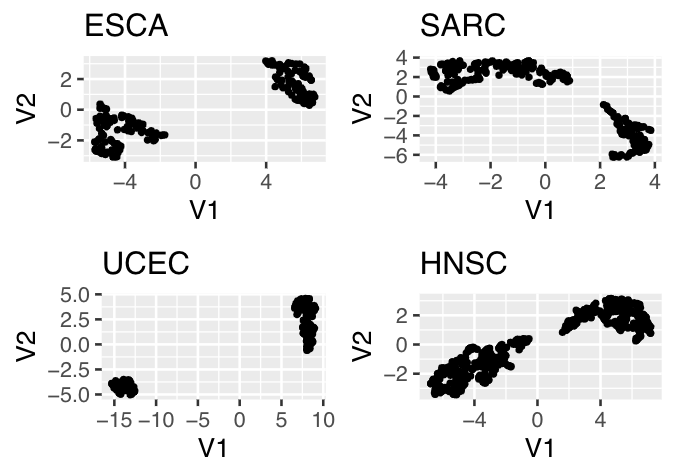
\includegraphics[width=9.44in]{figures/figure1} \caption{Title. Description}\label{fig:figure1}
\end{figure}

easier alternative: this is latex formatting. In Figure \ref{figure1}
you can see an UMAP. (+ label your figures, equations etc and then
reference with /\ref{})

\begin{figure}[htbp]
    \centering
    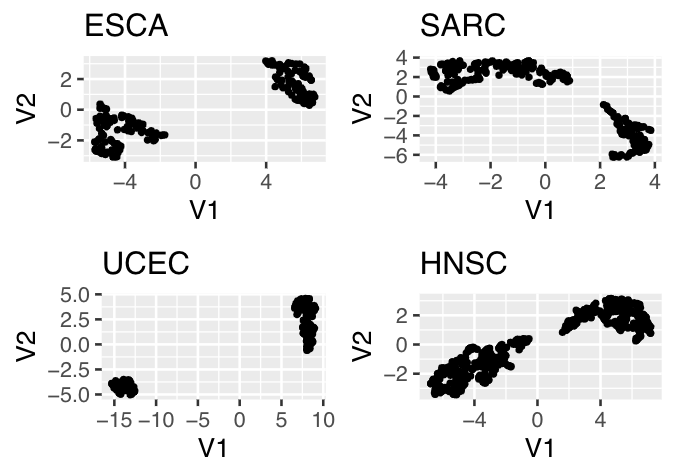
\includegraphics{figures/figure1.png}
    \caption[\textbf{Title}.]{\textbf{Title}. Description.}
    \label{figure1}
\end{figure}

\hypertarget{discussion}{%
\chapter{Discussion}\label{discussion}}

\hypertarget{immune-pathways-are-significantly-upregulated-in-x}{%
\section{Immune pathways are significantly upregulated in
X}\label{immune-pathways-are-significantly-upregulated-in-x}}

\hypertarget{references}{%
\chapter{References}\label{references}}

\hypertarget{refs}{}
\begin{CSLReferences}{0}{0}
\leavevmode\vadjust pre{\hypertarget{ref-kumar_multiple_2017}{}}%
Kumar, SK, Rajkumar, V, Kyle, RA, Duin, M van, Sonneveld, P, Mateos,
M-V, Gay, F, and Anderson, KC (2017). Multiple myeloma. Nat Rev Dis
Primers 3, 17046.

\leavevmode\vadjust pre{\hypertarget{ref-zavidij_single-cell_2020}{}}%
Zavidij, O et al. (2020). Single-cell {RNA} sequencing reveals
compromised immune microenvironment in precursor stages of multiple
myeloma. Nat Cancer 1, 493--506.

\end{CSLReferences}

\hypertarget{appendix}{%
\chapter{Appendix}\label{appendix}}

\hypertarget{plots}{%
\section{Plots}\label{plots}}

hello \#\# Code world

\begin{Shaded}
\begin{Highlighting}[]
\CommentTok{\#createn einer liste mit allen patienten in dfs sortiert nach krebs}
\NormalTok{cancers }\OtherTok{=} \FunctionTok{list}\NormalTok{();cancers }\OtherTok{=} \FunctionTok{vector}\NormalTok{(}\StringTok{\textquotesingle{}list\textquotesingle{}}\NormalTok{,}\FunctionTok{length}\NormalTok{(}\FunctionTok{table}\NormalTok{(tcga\_anno}\SpecialCharTok{$}\NormalTok{cancer\_type\_abbreviation)))}
\FunctionTok{names}\NormalTok{(cancers) }\OtherTok{=} \FunctionTok{names}\NormalTok{(}\FunctionTok{table}\NormalTok{(tcga\_anno}\SpecialCharTok{$}\NormalTok{cancer\_type\_abbreviation))}
\NormalTok{i}\OtherTok{=}\DecValTok{1}
\ControlFlowTok{for}\NormalTok{ (i }\ControlFlowTok{in} \DecValTok{1}\SpecialCharTok{:}\FunctionTok{length}\NormalTok{(cancers))\{}
\NormalTok{  cancers[[i]] }\OtherTok{=}\NormalTok{ tcga\_exp\_cleaned[,tcga\_anno}\SpecialCharTok{$}\NormalTok{cancer\_type\_abbreviation }\SpecialCharTok{==} \FunctionTok{names}\NormalTok{(cancers)[i]]}
\NormalTok{\}}
\CommentTok{\#function die einen krebstypen df und genesets als input nimmt und ein df mit pvalues ausgibt}
\NormalTok{enrichment }\OtherTok{=} \ControlFlowTok{function}\NormalTok{(expressiondata, }\AttributeTok{genesets =}\NormalTok{ genesets\_ids)\{}
\NormalTok{  ESmatrix }\OtherTok{=} \FunctionTok{sapply}\NormalTok{(genesets, }\AttributeTok{FUN =} \ControlFlowTok{function}\NormalTok{(x)\{}
\NormalTok{    ins }\OtherTok{=} \FunctionTok{na.omit}\NormalTok{(}\FunctionTok{match}\NormalTok{(x,}\FunctionTok{rownames}\NormalTok{(expressiondata)))}\CommentTok{\#indices der gene im aktuellen set}
\NormalTok{    outs }\OtherTok{=} \SpecialCharTok{{-}}\NormalTok{ins}\CommentTok{\#indices der gene nicht im aktuellen set}
    \CommentTok{\#gibt einen vektor der für jeden patienten den pval für das aktuelle gene enthält}
\NormalTok{    res }\OtherTok{=} \ConstantTok{NULL}
    \ControlFlowTok{for}\NormalTok{ (i }\ControlFlowTok{in} \DecValTok{1}\SpecialCharTok{:}\FunctionTok{ncol}\NormalTok{(expressiondata))\{}\CommentTok{\#testet für jeden patienten}
\NormalTok{      res[i] }\OtherTok{=} \FunctionTok{wilcox.test}\NormalTok{(expressiondata[ins,i],expressiondata[outs,i],}\StringTok{\textquotesingle{}two.sided\textquotesingle{}}\NormalTok{)}\SpecialCharTok{$}\NormalTok{p.value}
\NormalTok{    \}}
    \FunctionTok{return}\NormalTok{(res)}
\NormalTok{  \})}
  \FunctionTok{row.names}\NormalTok{(ESmatrix) }\OtherTok{=} \FunctionTok{colnames}\NormalTok{(expressiondata); }\FunctionTok{return}\NormalTok{(ESmatrix)}
\NormalTok{\}}
\NormalTok{pvalueslist }\OtherTok{=} \FunctionTok{lapply}\NormalTok{(cancers, enrichment)}\CommentTok{\#für die tests für jeden krebstypen durch}
\end{Highlighting}
\end{Shaded}

\begin{Shaded}
\begin{Highlighting}[]
\NormalTok{get\_top10pathways\_from\_pvalues }\OtherTok{=} \ControlFlowTok{function}\NormalTok{(df\_p\_values, length\_genesets) \{}
  
  \FunctionTok{require}\NormalTok{(ggplot2)}
  
\NormalTok{  results }\OtherTok{\textless{}{-}} \FunctionTok{list}\NormalTok{()}
    
\NormalTok{  df\_p\_values\_log10 }\OtherTok{\textless{}{-}} \SpecialCharTok{{-}}\FunctionTok{log10}\NormalTok{(}\FunctionTok{as.data.frame}\NormalTok{(df\_p\_values))}
    
\NormalTok{  mean\_pathway }\OtherTok{\textless{}{-}} \FunctionTok{as.data.frame}\NormalTok{(}\FunctionTok{apply}\NormalTok{(df\_p\_values\_log10, }\DecValTok{1}\NormalTok{, mean))}
  \FunctionTok{rownames}\NormalTok{(mean\_pathway) }\OtherTok{\textless{}{-}} \FunctionTok{rownames}\NormalTok{(df\_p\_values\_log10)}
  
\NormalTok{  ordered\_score }\OtherTok{\textless{}{-}}\NormalTok{ mean\_pathway[}\FunctionTok{order}\NormalTok{(}\SpecialCharTok{{-}}\NormalTok{mean\_pathway[ ,}\DecValTok{1}\NormalTok{]), }\DecValTok{1}\NormalTok{]}
\NormalTok{  top\_10 }\OtherTok{\textless{}{-}} \FunctionTok{data.frame}\NormalTok{(ordered\_score[}\DecValTok{1}\SpecialCharTok{:}\DecValTok{10}\NormalTok{])}
  \FunctionTok{colnames}\NormalTok{(top\_10) }\OtherTok{\textless{}{-}} \StringTok{"mean\_pathway"}
  
\NormalTok{  ordered\_names }\OtherTok{\textless{}{-}} \FunctionTok{order}\NormalTok{(}\SpecialCharTok{{-}}\NormalTok{mean\_pathway[ ,}\DecValTok{1}\NormalTok{])}
\NormalTok{  top\_10\_names }\OtherTok{\textless{}{-}}\NormalTok{ ordered\_names[}\DecValTok{1}\SpecialCharTok{:}\DecValTok{10}\NormalTok{]}
\NormalTok{  top\_10}\SpecialCharTok{$}\NormalTok{pathway\_names }\OtherTok{\textless{}{-}} \FunctionTok{row.names}\NormalTok{(mean\_pathway)[top\_10\_names]}
  
\NormalTok{  results[[}\DecValTok{1}\NormalTok{]] }\OtherTok{\textless{}{-}}\NormalTok{ top\_10}
  
\NormalTok{  results[[}\DecValTok{2}\NormalTok{]] }\OtherTok{\textless{}{-}} \FunctionTok{ggplot}\NormalTok{(}\AttributeTok{data =}\NormalTok{ top\_10, }\FunctionTok{aes}\NormalTok{(}\AttributeTok{x =}\NormalTok{ mean\_pathway, }\AttributeTok{y =} \FunctionTok{reorder}\NormalTok{(pathway\_names, mean\_pathway)))}\SpecialCharTok{+}
    \FunctionTok{geom\_bar}\NormalTok{(}\AttributeTok{stat =} \StringTok{"identity"}\NormalTok{)}\SpecialCharTok{+}
    \FunctionTok{coord\_cartesian}\NormalTok{(}\AttributeTok{xlim =}\FunctionTok{c}\NormalTok{(}\DecValTok{3}\NormalTok{, }\FloatTok{3.75}\NormalTok{))}\SpecialCharTok{+}
    \FunctionTok{labs}\NormalTok{(}\AttributeTok{title =} \FunctionTok{names}\NormalTok{(df\_p\_values),}
         \AttributeTok{x =} \StringTok{"mean p{-}value pathway"}\NormalTok{,}
         \AttributeTok{y =} \StringTok{"pathway name"}\NormalTok{)}
  
\NormalTok{  pathway\_size }\OtherTok{\textless{}{-}} \FunctionTok{order}\NormalTok{(}\SpecialCharTok{{-}}\NormalTok{mean\_pathway[ ,}\DecValTok{1}\NormalTok{])}
\NormalTok{  top\_10\_size }\OtherTok{\textless{}{-}}\NormalTok{ pathway\_size[}\DecValTok{1}\SpecialCharTok{:}\DecValTok{10}\NormalTok{]}
\NormalTok{  top\_10}\SpecialCharTok{$}\NormalTok{pathway\_size }\OtherTok{\textless{}{-}}\NormalTok{ length\_genesets[top\_10\_size]}
  
\NormalTok{  results[[}\DecValTok{3}\NormalTok{]] }\OtherTok{\textless{}{-}} \FunctionTok{ggplot}\NormalTok{(}\AttributeTok{data =}\NormalTok{ top\_10, }\FunctionTok{aes}\NormalTok{(}\AttributeTok{x =}\NormalTok{ mean\_pathway, }\AttributeTok{y =} \FunctionTok{reorder}\NormalTok{(pathway\_names,}
\NormalTok{                                                                          mean\_pathway)))}\SpecialCharTok{+}
    \FunctionTok{geom\_point}\NormalTok{(}\FunctionTok{aes}\NormalTok{(}\AttributeTok{size =}\NormalTok{ pathway\_size))}\SpecialCharTok{+}
    \FunctionTok{labs}\NormalTok{(}\AttributeTok{title =} \FunctionTok{names}\NormalTok{(df\_p\_values),}
         \AttributeTok{x =} \StringTok{"mean p{-}value pathway"}\NormalTok{,}
         \AttributeTok{y =} \StringTok{"pathway name"}\NormalTok{)}
  
  \FunctionTok{return}\NormalTok{(results)}
\NormalTok{\}}
\end{Highlighting}
\end{Shaded}


\end{document}
